\chapter{Mathematical Model}
\label{chp:MAT}
%%%%%%%%%%%%%%%%%%%%%%%%%%%%%%%%%%%%%%%%%%%%%%%%%%%%%%%%%%%%%%%%%%%%%%%
We will apply quantitative methods in order to achieve the objectives listed. Since we intend to study the contribution of the birth dose and treatment of infected mothers to the transmission dynamics of the disease, we will employ population-based deterministic ordinary differential equations(ODE) models which we will adapt and modify from the existing literature. Population-based deterministic models are proper at this stage since we are only interested in how the infected population structure behaves when the suggested interventions are applied. Other tools which are appropriate in achieving the objectives could include: delay differential equation models so as to introduce a delay in terms of various events such as the kick-start of immunity, a delay in taking the routine vaccination, and so on, or partial differential equations so as to set up our model implicitly in terms of age and/or time. However, this is outside the scope of our research question.

The model formulation process will take two ``stages":
In the first stage, an appropriate model from the literature will be adapted (and/or modified) to capture the contributions of the various interventions under investigation in our research questions \ref{sub question 1}, \ref{sub question 2} and \ref{sub question 3}. The interventions in questions \ref{sub question 1} and \ref{sub question 2} will be applied separately, and then combined, in order to answer question \ref{sub question 3}. This will help in identifying individual contributions of the interventions, as well as, the synergistic contribution.  These models will be simulated separately just as they have been described.  A simulation of the three separate models over time will then produce outputs which will be fed into the second stage. 

At stage two of the process, a sort of a ``reservoir'' will be created to keep track of the number of infants who remain infected after these interventions have been put in place. This output will flow into a larger population model for sub-Saharan Africa for simulation over several generations.  
The total contribution of HBV+ children into the larger population will thus be the foundation on which the hypothesis of eradication will be shown in this work.

\subsection{Model Framework}
We formulate a mathematical model to study the long term contribution of infected neonates to the general population-level infection dynamics. Our model studies the  impact of the administration of a birth and routine vaccine to infants, as well as treatment to infected pregnant women in sub-Saharan Africa where HBV is highly endemic.  

In our model, we assume that infants destined to take their first dose within 24 hours and the full routine vaccination within the next 6 months. This model serves as a feeder into a larger population model. It will feed the number of infants who remain infected (acute and chronic),  after several iterations, into the population model we shall develop.

To the best of our knowledge, not many models which consolidate HBV vertical transmission and two stages of vaccination have been published. In particular, none has been published, which studies the long term impact of combining a birth dose vaccine and a routine vaccine in the same model. 

To answer our research questions, we modify the models by \cite{mann2011modelling_NewZealand,zou2010modeling} by amalgamating ideas from the models in those papers. Of particular interest is the age-structured model by \cite{mann2011modelling_NewZealand}. We adapt the equation set (1) in \cite{mann2011modelling_NewZealand} for infants aged $0-1.25$ years since it captures the age structure of the neonates we intend to study, and modify it by including an extra dose of vaccination denoting the routine vaccination. For sub-question \ref{sub question 2}, we assume that there are two types of immunity induced in the infants for each stage of vaccination: for the birth dose, the infants acquire a temporary immunity which wanes. However, they acquire long term immunity if they proceed to receive the routine vaccination. The work by \cite{mclean1994modelling} extrapolated the vaccine-induced immunity period to be an average of 22.2 years from data which was collected over a period of 7 years. This vaccine-induced immunity acquired by these infants, we assume, is comparable to that acquired by the carrier individuals who clear the infection. This assumption is in contradiction to that of the model of \cite{zou2010modeling}. Our assumption is, however, justifiable since we only intend to simulate our model over a number of generations which amounts to a time period less than the average vaccine-induced immunity duration. It is therefore safe to equate the two types of acquired immunities described in our model and classify those two groups of individuals into the same epidemiological group. Again, in agreement with \cite{zhang2012analysisHBVmodel}, we assume that all infants born infected will be classified as chronic carriers. Finally, in accordance with \cite{mann2011modelling_NewZealand}, our model assumes that HBV-related deaths in the birth cohort in totality are negligible.


The model flowchart in Figure \ref{fig:flowchart} describes a modified SIR type model. The model consists of the following class of individuals, all of whom are neonates within their first 24 hours of birth: susceptible babies, $S_b,$ infants who receive the routine vaccine, $V_b,$ chronically infected babies, $I_b, $  and those with full immunity either by receving the vaccine or through natural clearance, $R_b$ .

\section{Model Assumptions}
The following simplifying assumptions were made in the model below:
\begin{enumerate}
	\item There are constant inflows or births. 
	\item Babies are either born infected or susceptible. We classify all infected babies as chronic in agreement with \cite{zhang2012analysisHBVmodel}.
	\item There is an existing routine vaccination in place.
	\item Babies are only infected through vertical transmission, either before or after birth. Horizontal transmission is ignored at this stage.
	\item Since the time it takes for infants to become chronic is very short compared to the time span of infected, it is assumed all the infected infants are chronic.
	\item The routine vaccine provides permanent immunity.
	\item All the babies are at equal risk of acquiring the infection.
	\item There is no HBV related mortality at that stage.
	
\end{enumerate}

\subsubsection{Flowchart Description}
Neonates are either born susceptible or infected and that is how $S$ and $I$ are populated. A proportion of the susceptible individuals receive the routine vaccine after birth, moving to $V$ .  The rest get infected vertically and move to $I$. The infants who receive the routine vaccine will populate the $R$ compartment with full protection after immunity kicks in. The infants who clear the infection naturally will move to $R$ as well. 
\clearpage 		
The model flow diagram is represented in Figure \ref{fig:flowchart}. 
\begin{figure}[h!]
	\centering
	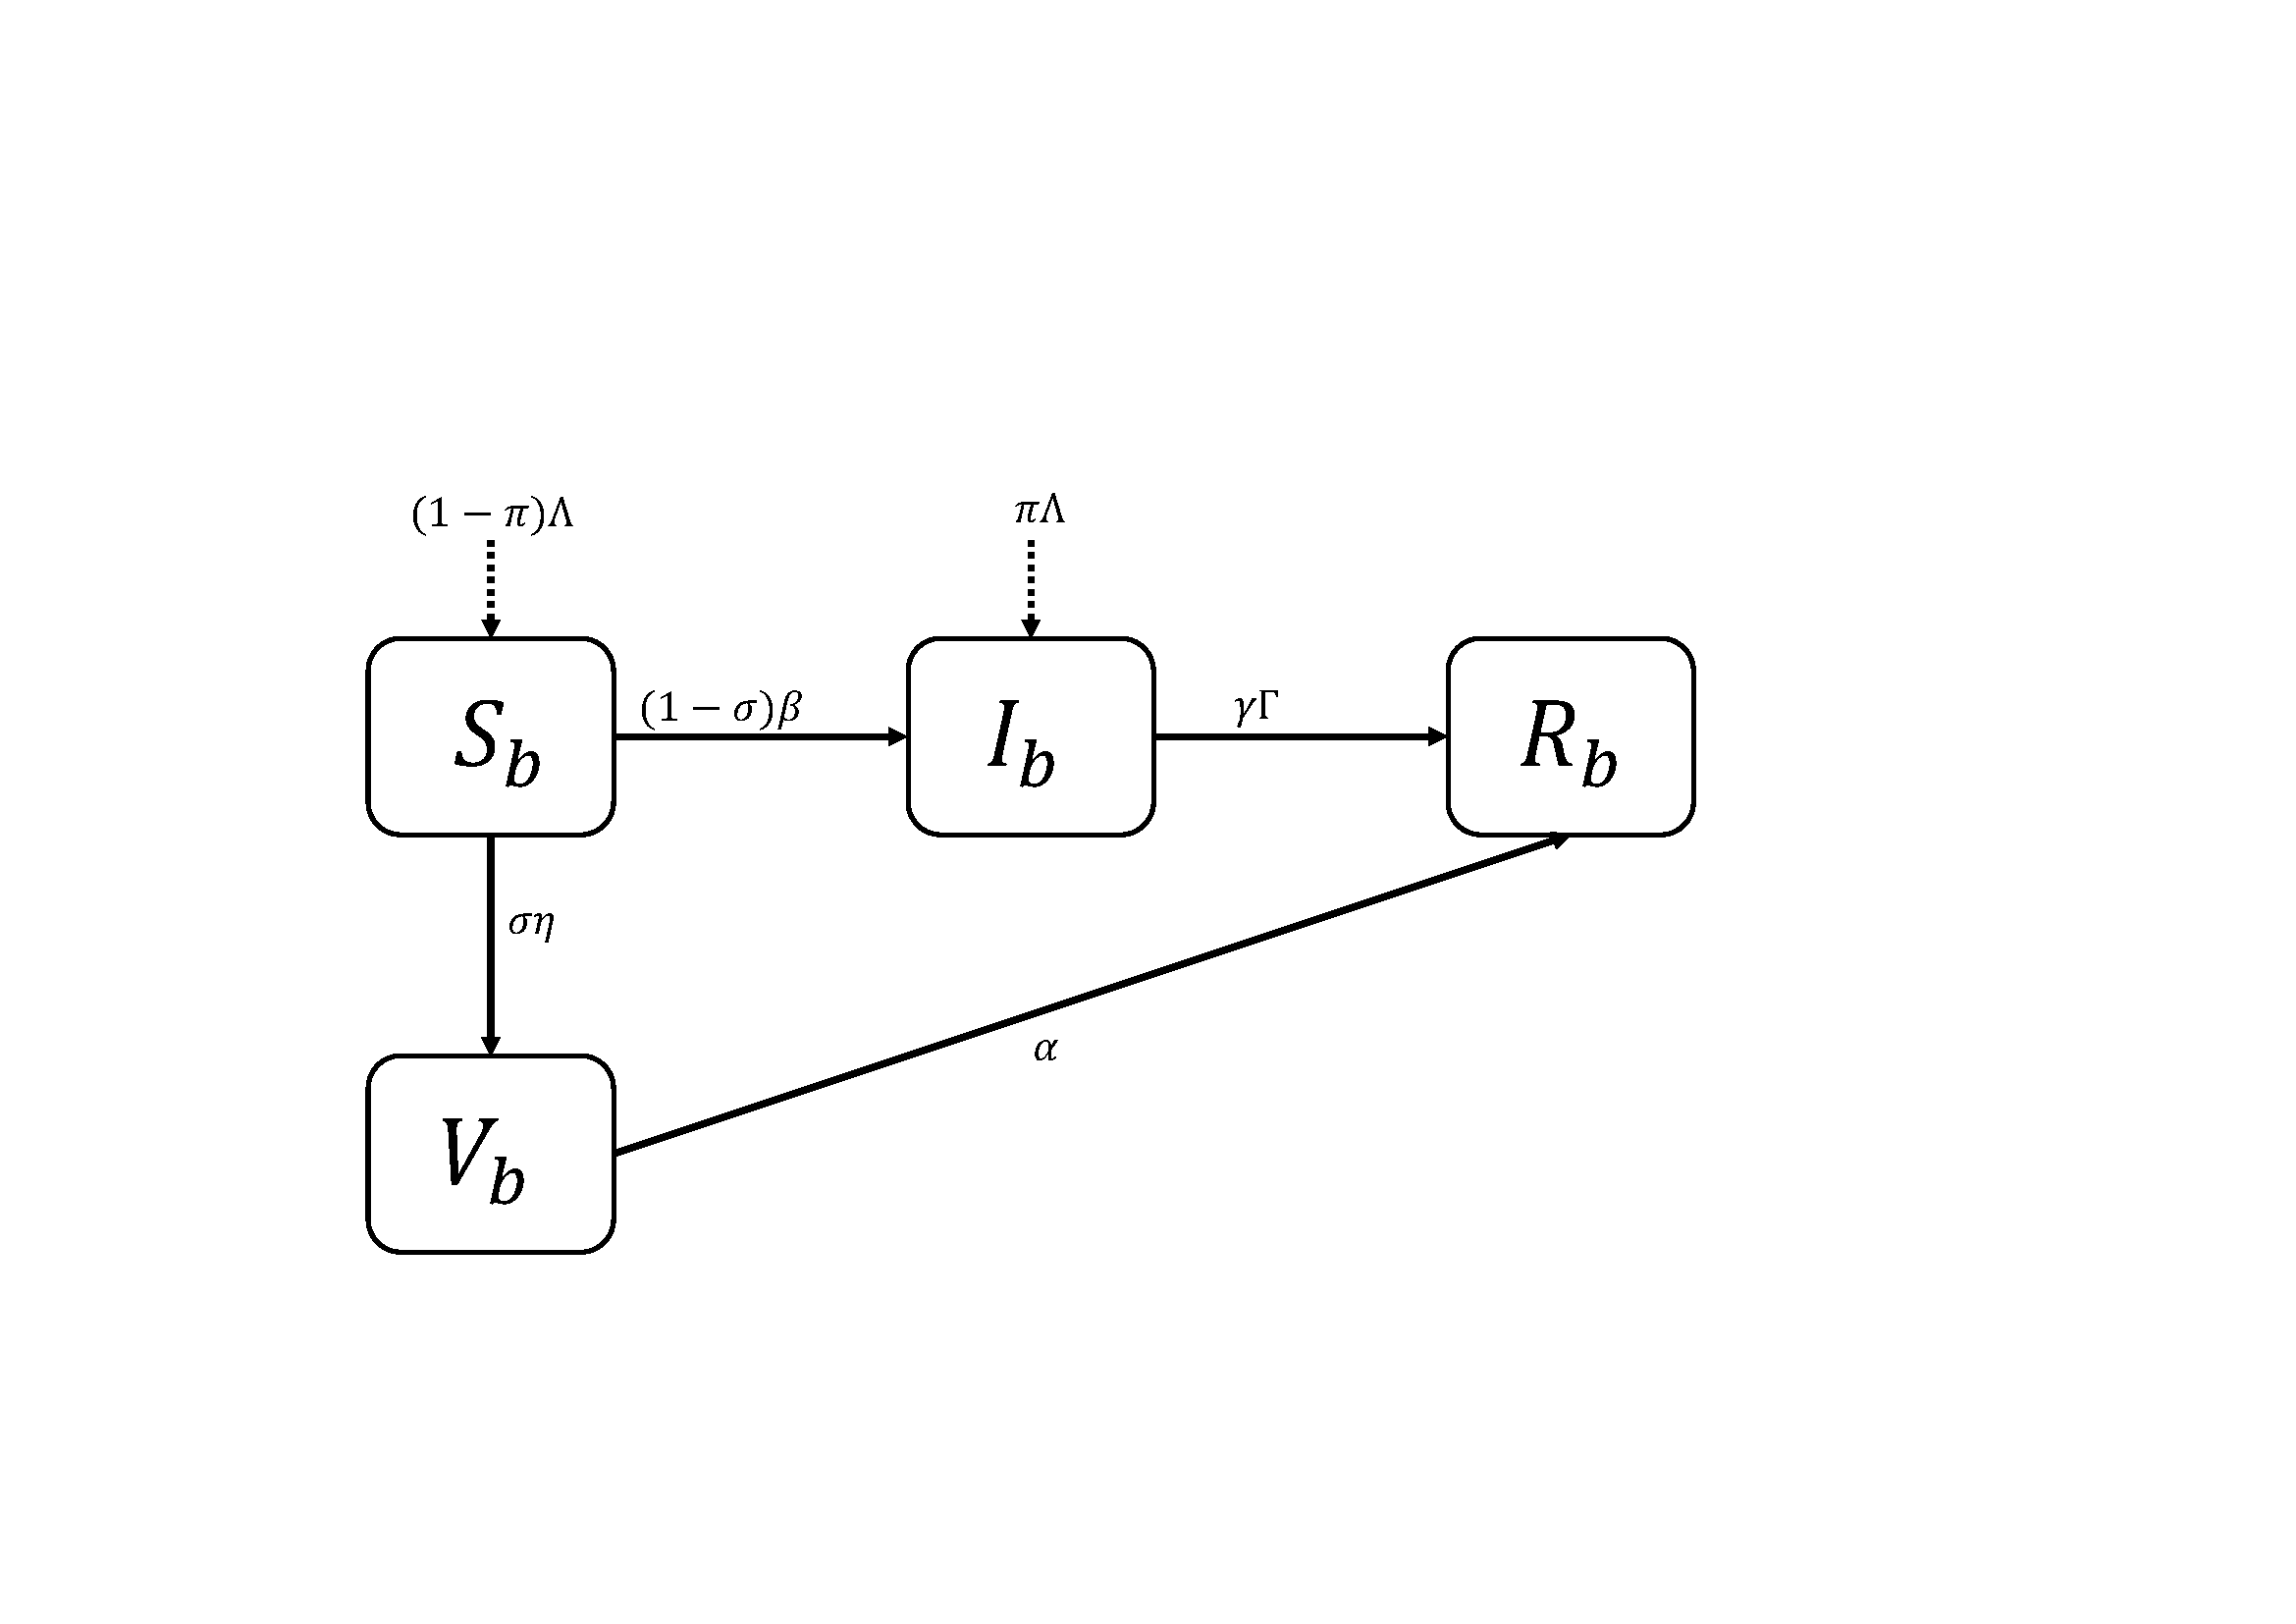
\includegraphics[scale=0.65]{NewModel.png}
	\caption{the SVIR model structure indicating vertical transmission. The solid arrows indicate movement of the individuals, whiles the dashed arrows represent initial inflows.} \label{fig:flowchart}
\end{figure}

The systems of ordinary differential equations representing the dynamics described above are as follows:
\begin{align}
\begin{split}
\dfrac{dS}{dt}&=(1-\pi)\Lambda -\beta S_b(\frac{I_m+C_m}{N_m})-\sigma\eta-muS_b,\\
\dfrac{dV}{dt}&=\sigma\eta S_b-(\mu+\alpha) V_b\\
\dfrac{dI}{dt}&=\beta S_b(\frac{I_m+C_m}{N_m}) + \pi\Lambda-\gamma\Gamma-\mu I_b,\\
\dfrac{dR}{dt}&=\sigma\eta S - (\mu +\alpha) V_b.
\end{split}
\end{align}
The various parameters used in our model are described the following table:

\vspace{1cm}
\begin{table}[h]
	\centering
	\begin{tabular}{ |p{1.57cm}|p{10cm}|p{2cm}| }
		\hline
		Parameter& Description &    Source \\
		\hline
		$\Lambda$    		& 	Total births per year  					&																																								\\
		$	\mu $					&  	natural death rate   &																																									\\
		$\beta$ 					& 	mother-to-child contact rate &																																			\\
		$\gamma$ 			& 	rate of natural clearance of infection										&																							\\
		$\alpha$ 				& 	rate of acquiring vaccine-induced permanent immunity	&																								\\
		$\eta  $					& routine vaccination rate																&																								\\
		$\sigma$ 				& 	proportion of infants who receive the routine vaccine &																							\\
		$\Gamma$			& 	Proportion of infected babies who clear naturally		&																						\\
		\hline
	\end{tabular}
	\caption{Model parameters and their descriptions}
	\label{table:1}
	
	
		\centering
		\begin{tabular}{ |p{1.57cm}|p{12cm}| }
			\hline
			Group & Description \\
			\hline
			$	S		$    		& 		Susceptible to the infection    \\
			$	V 		$			&  	 	Infants with the routine vaccination	\\
			$	I 		$			&  	 	Chronically infected babies   		\\
			$	R		$ 			& 		Fully immune individuals		\\
			\hline
		\end{tabular}
		\caption{Description of epidemiological grouping}
		\label{table:2}
		\vspace{1mm}
\end{table}
